% Figure 1: the figures a report prints, and the table they determine.
% House vocabulary: HOUSE_STYLE/docs/viz.md. Compile: pdflatex fig_recovery.tex
\documentclass[tikz,border=6pt]{standalone}
\usepackage{amsmath,amssymb}
\usetikzlibrary{arrows.meta,positioning,calc,fit,backgrounds}

\definecolor{boxblue}{HTML}{DBEAFE}   \definecolor{bordblue}{HTML}{3B82F6}
\definecolor{boxgreen}{HTML}{D1FAE5}  \definecolor{bordgreen}{HTML}{059669}
\definecolor{boxred}{HTML}{FEE2E2}    \definecolor{bordred}{HTML}{DC2626}
\definecolor{anncolor}{HTML}{6B7280}
\definecolor{ink}{HTML}{1B2A41}

\begin{document}
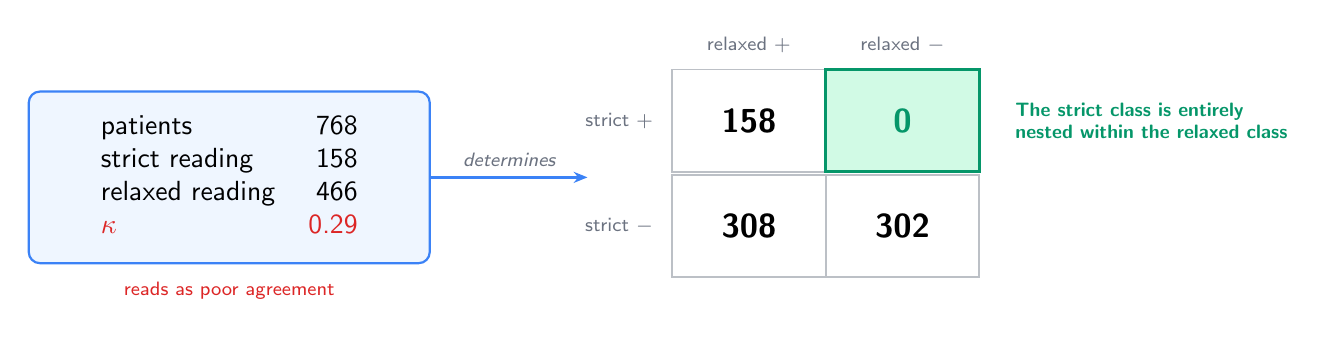
\begin{tikzpicture}[
    font=\sffamily,
    box/.style={rectangle, rounded corners=4pt, text centered,
                line width=0.8pt, inner sep=7pt},
    printbox/.style={box, draw=bordblue, fill=boxblue!45, text width=4.6cm},
    cell/.style={rectangle, minimum width=1.95cm, minimum height=1.3cm,
                 text centered, font=\sffamily\bfseries\large,
                 draw=anncolor!45, line width=0.7pt, fill=white},
    keycell/.style={cell, draw=bordgreen, fill=boxgreen, text=bordgreen, line width=1.1pt},
    hdr/.style={font=\sffamily\scriptsize, color=anncolor},
    ann/.style={font=\sffamily\scriptsize, color=anncolor, align=left},
    onarrow/.style={font=\sffamily\scriptsize\itshape, color=anncolor},
    arr/.style={-{Stealth[length=5pt,width=4pt]}, line width=1.1pt, color=#1},
]

\node[printbox] (printed) at (0,0)
    {\begin{tabular}{@{}l@{\hspace{12pt}}r@{}}
     patients & 768\\
     strict reading & 158\\
     relaxed reading & 466\\
     \textcolor{bordred}{$\kappa$} & \textcolor{bordred}{0.29}
     \end{tabular}};
\node[ann, below=3pt of printed.south, anchor=north] {\textcolor{bordred}{reads as poor agreement}};

\node[cell] (c11) at (6.6,0.72) {158};
\node[keycell] (c10) at (8.55,0.72) {0};
\node[cell] (c01) at (6.6,-0.62) {308};
\node[cell] (c00) at (8.55,-0.62) {302};
\node[hdr, above=2pt of c11] {relaxed $+$};
\node[hdr, above=2pt of c10] {relaxed $-$};
\node[hdr, left=3pt of c11] {strict $+$};
\node[hdr, left=3pt of c01] {strict $-$};
\draw[arr=bordblue] (printed.east) -- node[onarrow, above] {determines} (4.55,0);

\node[ann, right=9pt of c10]
    {\textcolor{bordgreen}{\bfseries The strict class is entirely}\\
     \textcolor{bordgreen}{\bfseries nested within the relaxed class}};

\end{tikzpicture}
\end{document}
